\documentclass{article}
\usepackage{graphicx}
\usepackage[utf8]{inputenc}
\usepackage{listings}
\usepackage{color}
\usepackage{xcolor}
\usepackage{textcomp}
\usepackage{amsmath}
\usepackage{mathabx}

\definecolor{solarized@base03}{HTML}{002B36}
\definecolor{solarized@base02}{HTML}{073642}
\definecolor{solarized@base01}{HTML}{586e75}
\definecolor{solarized@base00}{HTML}{657b83}
\definecolor{solarized@base0}{HTML}{839496}
\definecolor{solarized@base1}{HTML}{93a1a1}
\definecolor{solarized@base2}{HTML}{EEE8D5}
\definecolor{solarized@base3}{HTML}{FDF6E3}
\definecolor{solarized@yellow}{HTML}{B58900}
\definecolor{solarized@orange}{HTML}{CB4B16}
\definecolor{solarized@red}{HTML}{DC322F}
\definecolor{solarized@magenta}{HTML}{D33682}
\definecolor{solarized@violet}{HTML}{6C71C4}
\definecolor{solarized@blue}{HTML}{268BD2}
\definecolor{solarized@cyan}{HTML}{2AA198}
\definecolor{solarized@green}{HTML}{859900}

\lstset{
  language=Python,
  upquote=true,
  columns=fixed,
  tabsize=2,
  extendedchars=true,
  breaklines=true,
  frame=single,
  numbers=left,
  numbersep=5pt,
  rulesepcolor=\color{solarized@base03},
  numberstyle=\tiny\color{solarized@base01},
  basicstyle=\footnotesize\ttfamily,
  keywordstyle=\color{solarized@green},
  stringstyle=\color{solarized@cyan}\ttfamily,
  identifierstyle=\color{solarized@blue},
  commentstyle=\color{solarized@base01},
  emphstyle=\color{solarized@red}
}
\begin{document}

\title{Tarea Método de Punto Fijo}
\author{Angel Caceres Licona}

\maketitle

\section{Considerar la función $e^x+x^2-x-4$...}
\subsection{Construya tresdiferentes funciones de iteracion.}
Consideremos primero $g(x)=e^x+x^2-4$

Gráfica de la primer $g(x)$

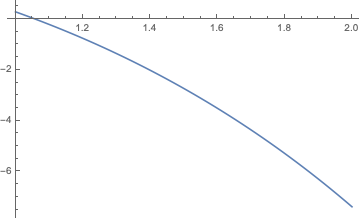
\includegraphics[scale=0.4]{grafica1ergx.png}

La derivada de esta función es:

$g'(x) = -e^x-2x$ 
y tenemos que
$|g'(x)| < 1$ para $x \in (-0.74, 0)$

Al hacer las iteraciones obtenemos lo siguiente:

\begin{center}
    \begin{tabular}{||c c||} 
    \hline
    $n$ & $g(x)$\\ [0.5ex] 
    \hline
    1 & -0.281718171541 \\
    \hline
    2 & -3.16614858154 \\
    \hline
    3 & 6.06666252367 \\
    \hline
    4 & 464.043421299 \\ 
    \hline
    5 & 3.40014339901e+201 \\ [1ex]
    \hline

   \end{tabular}
\end{center}
Que no converge a la raíz buscada.

Probamos con una segunda $g(x) = \log( -x^2 + x +4)$
Su derivada es $g'(x)\frac{1-2x}{-x^2+x+4}$
Y tenemos que $|g'(x)|<1$ no tiene soluciones reales.
Iteramos y obtenemos lo siguiente:

\begin{center}
    \begin{tabular}{||c c||} 
    \hline
    $n$ & $g(x)$\\ [0.5ex] 
    \hline
    1 & 1.38629436112 \\
    \hline
    2 & 1.24256321468 \\
    \hline
    3 & 1.30795433512 \\
    \hline
    4 & 1.28015848727 \\ 
    \hline
    5 & 1.29235524303 \\
    \hline
    6 & 1.2870741686 \\
    \hline
    7 & 1.28837503694 \\
    \hline
    8 & 1.28880963902\\
    \hline
    9 & 1.2886207127 \\ 
    \hline
    10 & 1.28870285824 \\ [1ex]
    \hline
   \end{tabular}
\end{center}

Que parece estar convergiendo muy lentamente.

Escogemos una tercera $g(x)= \frac{-e^x+x+4}{x}$
Tenemos que $g'(x) = - \frac{e^x(x-1)+4}{x^2}$
y que $|g'(x)|<1 x \in (-1.88751, 0)$

Iteramos y obtenemos lo siguiente

\begin{center}
    \begin{tabular}{||c c||} 
    \hline
    $n$ & $g(x)$\\ [0.5ex] 
    \hline
    1 & 2.28171817154  \\
    \hline
    2 & -1.53909222227 \\
    \hline
    3 & -1.45951746429 \\
    \hline
    4 & -1.58143648714 \\ 
    \hline
    5 & -1.39928735729 \\
    \hline
    6 & -1.68224194147 \\
    \hline
    7 & -1.26723832134 \\
    \hline
    8 & -1.93424818125\\
    \hline
    9 & -0.993263918688 \\ 
    \hline
    10 & -2.65424944943 \\ [1ex]
    \hline
   \end{tabular}
\end{center}

que tampoco converge.

\section{Código del programa}

\begin{lstlisting}
from math import *


def gx(x):
    return -exp(x) -x**2 +4

def puntofijo(a,tol, n = 20):

    i = 1
    b = gx(a)
    tramo = abs(b-a)
    while(tramo>=tol and i<=n):
        print "El punto fijo es ",b," despues de ",i," iteraciones"
        a = b
        b = gx(a)
        tramo = abs(b-a)
        i = i+1
    respuesta = b

    return(respuesta)

respuesta = puntofijo(-0.74,10**-25)
\end{lstlisting}

\section{Repetir el ejercicio con $x^3-x^2-10x+7$}
Primero graficamos en el intervalo $(0,1)$
\begin{center}
    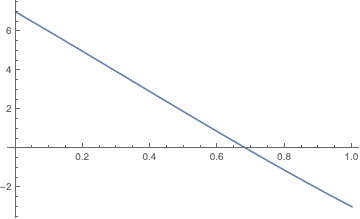
\includegraphics[scale=0.75]{grafica2.png}
\end{center}
Probamos la primer $g(x)= \frac{x^3-x^2+7}{10}$ y obtenemos
\begin{center}
    \begin{tabular}{||c c||} 
    \hline
    $n$ & $g(x)$\\ [0.5ex] 
    \hline
    1 & 0.6991 \\
    \hline
    2 & 0.685293789027 \\
    \hline
    3 & 0.685220528459 \\ [1ex]
    \hline
   \end{tabular}
\end{center}
que convergió rápido.

Probamos la segunda $g(x)= \frac{x^3-10x+7}{x}$ y obtenemos
\begin{center}
    \begin{tabular}{||c c||} 
    \hline
    $n$ & $g(x)$\\ [0.5ex] 
    \hline
    1 & 60.01 \\
    \hline
    2 & 3591.31674723 \\
    \hline
    3 & 12897545.9809 \\ 
    \hline
    2 & 1.66346692328e+14 \\
    \hline
    2 & 2.76712220485e+28 \\
    \hline
    2 & 7.65696529659e+56 \\
    \hline
    2 & 5.86291175531e+113 \\ [1ex]
    \hline
   \end{tabular}
\end{center}
que no converge.

Probamos con una tercera $g(x) = \sqrt{x^3-10x+7}$ y obtenemos que el programa truena por intentar calcular una raíz de un numero negativo.

\section{Repetir el ejercicio con $f(x) = 1.05 - 1.04x +\log(x)$}
Primero graficamos en el intervalo $(1,2)$
\begin{center}
    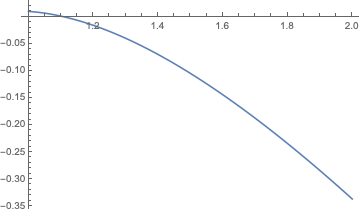
\includegraphics[scale=0.75]{grafica3.png}
\end{center}

Probamos la primer $g(x)= \frac{1.05 + \log(x)}{1.04}$ y obtenemos

\begin{center}
    \begin{tabular}{||c c||} 
    \hline
    $n$ & $g(x)$\\ [0.5ex] 
    \hline
    1 & 1.00961538462 \\
    \hline
    2 & 1.01881677982 \\
    \hline
    3 & 1.02754032132 \\ 
    \hline
    2 & 1.03573837382 \\
    \hline
    2 & 1.04337940099 \\
    \hline
    2 & 1.05044698962 \\
    \hline
    2 & 1.05693824807 \\ [1ex]
    \hline
   \end{tabular}
\end{center}

que converge lentamente.
Probamos una segunda $g(x) = e^{-1.05 + 1.04x}$ y obtenemos lo siguiente:

\begin{center}
    \begin{tabular}{||c c||} 
    \hline
    $n$ & $g(x)$\\ [0.5ex] 
    \hline
    1 & 0.990049833749 \\
    \hline
    2 & 0.979857454096 \\
    \hline
    3 & 0.969525746926 \\ 
    \hline
    2 & 0.959163984704 \\
    \hline
    2 & 0.948883303392 \\
    \hline
    2 & 0.938791973795 \\
    \hline
    2 & 0.928990889263 \\ [1ex]
    \hline
   \end{tabular}
\end{center}
que tampoco converge

\section{Clasifique las funciones por rapidez de convergencia...}
\begin{center}
    \begin{tabular}{||c c c c c||} 
    \hline
    $n$ & $g_1(x)$ & $g_2(x)$ & $g_3(x)$ & $g_4(x)$ \\ [0.5ex] 
    \hline
    1 & 2.64575131106 & diverge rápido  & 2.1573526803 & 1.50747491667 \\
    \hline 
    2 & 2.31392495318 & . & 2.12927784776 & 1.80533262168 \\
    \hline 
    3 & 2.085113115356 & . & 2.10345737732 & 1.89833372223 \\ 
    \hline 
    4 & 1.96790027706 & . & 2.05854241047 & 1.91158621947 \\
    \hline 
    5 & 1.92672978417& . & 2.03934932642 & 1.91281576256 \\
    \hline 
    6 & 1.9160343453 & . & 2.02221852111 & 1.91292134565 \\
    \hline 
    7 & 1.9136073772 & . & 2.0070346352 & . \\ 
    \hline
    8 & 1.91307744943 & . & 1.99366482238 & . \\
    \hline 
    9 & 1.91296277044 & . & 1.98196454838 & .\\
    \hline 
    10 & 1.91293800204 & . & 1.9717832322 & .\\
    \hline 
    11 & . & . & 1.9629693429 & .\\
    \hline 
    12 & . & . & 1.95537469059 & .\\
    \hline 
    13 & . & . & 1.94885778226 & .\\
    \hline 
    14 & . & . & 1.94328622775 & .\\
    \hline 
    15 & . & . & 1.93853826786 & .\\
    \hline 
    16 & . & . & 1.9345035497 & .\\
    \hline 
    17 & . & . & 1.93108329847 & .\\ [1ex]
    \hline 
   \end{tabular}
\end{center}

Entonces vemos que la que converge mas rápido es $g(x) = x- \frac{x^3 - 7}{12}$

\end{document}